\documentclass{scrreprt}
\usepackage[english]{babel}
\usepackage[T1]{fontenc}
\usepackage{lmodern}
\usepackage{blindtext}
\usepackage[utf8]{inputenc}
\usepackage{siunitx} %For unit handling%
\renewcommand{\familydefault}{\sfdefault}
\newcommand{\unit}[1]{\ensuremath{\, \mathrm{#1}}}
\usepackage{amssymb, amsmath, cancel, ulem, graphicx, float, tabularx, multirow, bm}
\usepackage{amsmath}

\setcounter{secnumdepth}{5}
\setcounter{tocdepth}{5}

\renewcommand{\emph}[1]{\textit{#1}}

\author{Urs Gerber\\09-921-156 \and Gian-Luca Mateo\\11-113-545}
\date{14th of March 2013}

\title{Collision Experiment}
\subtitle{Practical course report}

\begin{document}

\maketitle

\tableofcontents
\newpage

\chapter{Experiment: Momentum Conservation}
\section{Introduction}
A collision is a short-time interaction between two or more objects. In essence there are two types of collisions: the \emph{elastic} collision and the \emph{inelastic} collision.\\
In an ideal \emph{elastic} collision no energy is lost during the course of the interaction, meaning no energy is lost due to heat or deformation. In this type of collision both energy and momentum are conserved.\\
In the inelastic case both bodies will stick to each other after the collision and travel at a common terminal velocity. Only momentum is conserved as energy is lost to deformation.
 
\subsection{Goal of the experiment}

\subsection{Theory}
\subsubsection{Preliminary exercises}
Using $A:=\frac{m_2}{m_1}$

\paragraph*{Task 1}
\begin{equation}
m_1v_1=m_1v_1'+m_2v_2'
\end{equation}
\begin{equation}
\Rightarrow v_2'=\frac{m_1}{m_2}(v_1-v_1')
\end{equation}
\begin{equation}
\frac{1}{2}m_1v_1^2=\frac{1}{2}m_1v_1'^2+\frac{1}{2}m_2v_2'^2
\end{equation}
\begin{equation}
\Rightarrow m_1v_1^2=m_1v_1'^2+\frac{m_1^2}{m_2}(v_1-v_1')^2
\end{equation}
\begin{equation}
\Rightarrow v_1^2=v_1'^2+\frac{m_1}{m_2}(v_1-v_1')^2
\end{equation}
\begin{equation}
\Rightarrow v_1^2-v_1^2=\frac{m_1}{m_2}(v_1-v_1')^2
\end{equation}
\begin{equation}
\Rightarrow (v_1+v_1')=\frac{m_1}{m_2}(v_1-v_1')
\end{equation}
\begin{equation}
\Rightarrow v_1+v_1'=\frac{1}{A}(v_1-v_1')
\end{equation}
\begin{equation}
\Rightarrow v_1-\frac{v_1}{A}=-v_1-\frac{v_1'}{A}
\end{equation}
\begin{equation}
\Rightarrow v_1\left(1-\frac{1}{A}\right)=-v_1'\left(1+\frac{1}{A}\right)
\end{equation}
\begin{equation}
\Rightarrow \frac{v_1'}{v_1}=-\frac{1-\frac{1}{A}}{1+\frac{1}{A}} = \frac{A-1}{-A-1}
\end{equation}
\begin{equation}
\Rightarrow \frac{T_1'}{T_1} = \left(\frac{A-1}{-(A+1)}\right)^2=\left(\frac{A-1}{A+1}\right)^2
\end{equation}

\paragraph*{Task 2}
\begin{equation}
\frac{T_{1,2}'}{T_1}=\frac{(m_1+m_2)v_1'^2}{m_1v_1^2}
\end{equation}
\begin{equation}
v_1'=v_1\frac{m_1}{m_1+m_2}
\end{equation}
\begin{equation}
\Rightarrow \frac{T_1'}{T_1}= \frac{(m_1+m_2)}{m_1}\frac{v_1^2\left(\frac{m_1}{m_1+m_2}\right)^2}{v_1^2}=\frac{m_1}{m_1+m_2}=\frac{1}{1+A}
\end{equation}
\begin{equation}
\Rightarrow \frac{Q}{T_1}=1-\frac{T_1'}{T_1}=1-\frac{1}{1+A}=\frac{A}{1+A}
\end{equation}
Q is the fraction of the energy of $T_1$ lost in the collision. Q is composed of thermic energy, deformation energy and sound.

\paragraph*{Task 3}
\begin{equation}
l^2=a^2+(l-h)^2=a^2+l^2-2lh+\underbrace{h^2}_{\approx 0}
\end{equation}
\begin{equation}
\Rightarrow h=\frac{a^2}{2l}
\end{equation}
\begin{equation}
\frac{1}{2}m_2v_2'^2=m_2gh_2 \mbox{ und } \frac{1}{2}m_1v_1^2=m_1gh_1
\end{equation}
\begin{equation}
\frac{T_2'}{T_1}=\frac{m_2gh_2}{m_1gh_1}=\frac{m_2\frac{a_2^2}{2l}}{m_1\frac{a_1^2}{2l}}=\frac{m_2a_2^2}{m_1a_1^2}=A\frac{a_2^2}{a_1^2}
\end{equation}

\paragraph*{Task 4}
\begin{figure}[H]
	\centering
  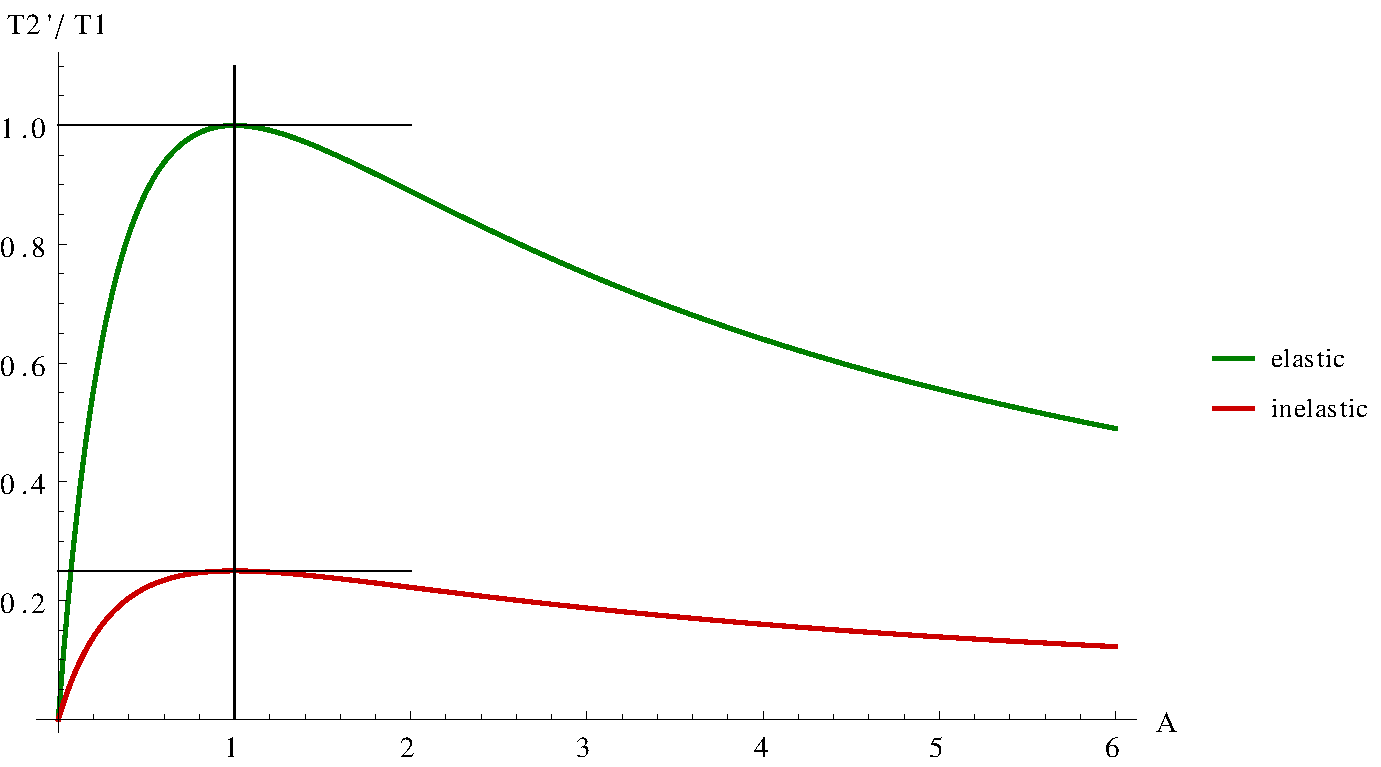
\includegraphics[width=0.9\textwidth]{diag/collision.pdf}
	\caption{$\frac{T_2'}{T_1}$ in dependance of $A$}
	\label{fig:task4}
\end{figure}
\noindent Figure \ref{fig:task4} shows the progression of $\frac{T_2'}{T_1}$ dependance of $A$ for an elastic and inelastic collision.\\
One can easily see that the maximum transfer of energy occurs at $A=1\Leftrightarrow m_1=m_2$

\paragraph*{Task 5}
We need the following formulae to analyze our data:
\begin{center}
\begin{tabular}{lrl}
Theory, elastic & $\frac{T_2'}{T_1} = $ &  $\frac{4A}{(A+1)^2}$ \\
Theory, inelastic &$\frac{T_2'}{T_1} =$ &  $\frac{A}{(A+1)^2}$ \\
Measurment & $\frac{T_2'}{T_1} = $ & $A \frac{a_2^2}{a_1^2}$ \\
Theory & $\frac{Q}{T_1} = $ & $\frac{A}{1+A}$ \\
Measurement & $\frac{Q}{T_1} =$ & $1-(1+A)\frac{a_2^2}{a_1^2}$ \\
\end{tabular}
\end{center}

\subsection{Uncertainty analysis}
\subsubsection{Kinetic Energy}
\begin{equation}
\frac{T_2'}{T_1}=A\frac{a_2^2}{a_1^2}\doteq t(a_1,a_2)
\end{equation}
\begin{align}
f(x,y) \doteq A\frac{y^2}{x^2} \Longrightarrow
s_f^2 &= \left(\frac{\partial f}{\partial x}\right)^2 s_x^2 + \left(\frac{\partial f}{\partial y}\right)^2 s_y^2\\
&= 4 A^2 \left( \frac{y^4}{x^6} s_x^2 + \frac{y^2}{x^4} s_y^2 \right)
\end{align}
\begin{equation}
\Longrightarrow s_{\bar{t}}^2 = 4 A^2 \left(\frac{\overline{a_2}^4}{\overline{a_1}^6} s_{\overline{a_1}}^2 + \frac{\overline{a_2}^2}{\overline{a_1}^4} s_{\overline{a_2}}^2 \right)
\end{equation}

\subsubsection{Energy Loss}
\begin{equation}
\frac{Q}{T_1}= 1-(1+A) \frac{a_2^2}{a_1^2} \doteq q(a_1,a_2)
\end{equation}
\begin{align}
f(x,y) \doteq A\frac{y^2}{x^2} \Longrightarrow
s_f^2 &= \left(\frac{\partial f}{\partial x}\right)^2 s_x^2 + \left(\frac{\partial f}{\partial y}\right)^2 s_y^2\\
&= 4 A^2 \left( \frac{y^4}{x^6} s_x^2 + \frac{y^2}{x^4} s_y^2 \right)
\end{align}
\begin{equation}
\Longrightarrow s_{\bar{q}}^2 = 4 A^2 \left(\frac{\overline{a_2}^4}{\overline{a_1}^6} s_{\overline{a_1}}^2 + \frac{\overline{a_2}^2}{\overline{a_1}^4} s_{\overline{a_2}}^2 \right)
\end{equation}

\section{Experiment setup and execution}

\subsection{Used materials}
\begin{figure}[H]
	\centering
  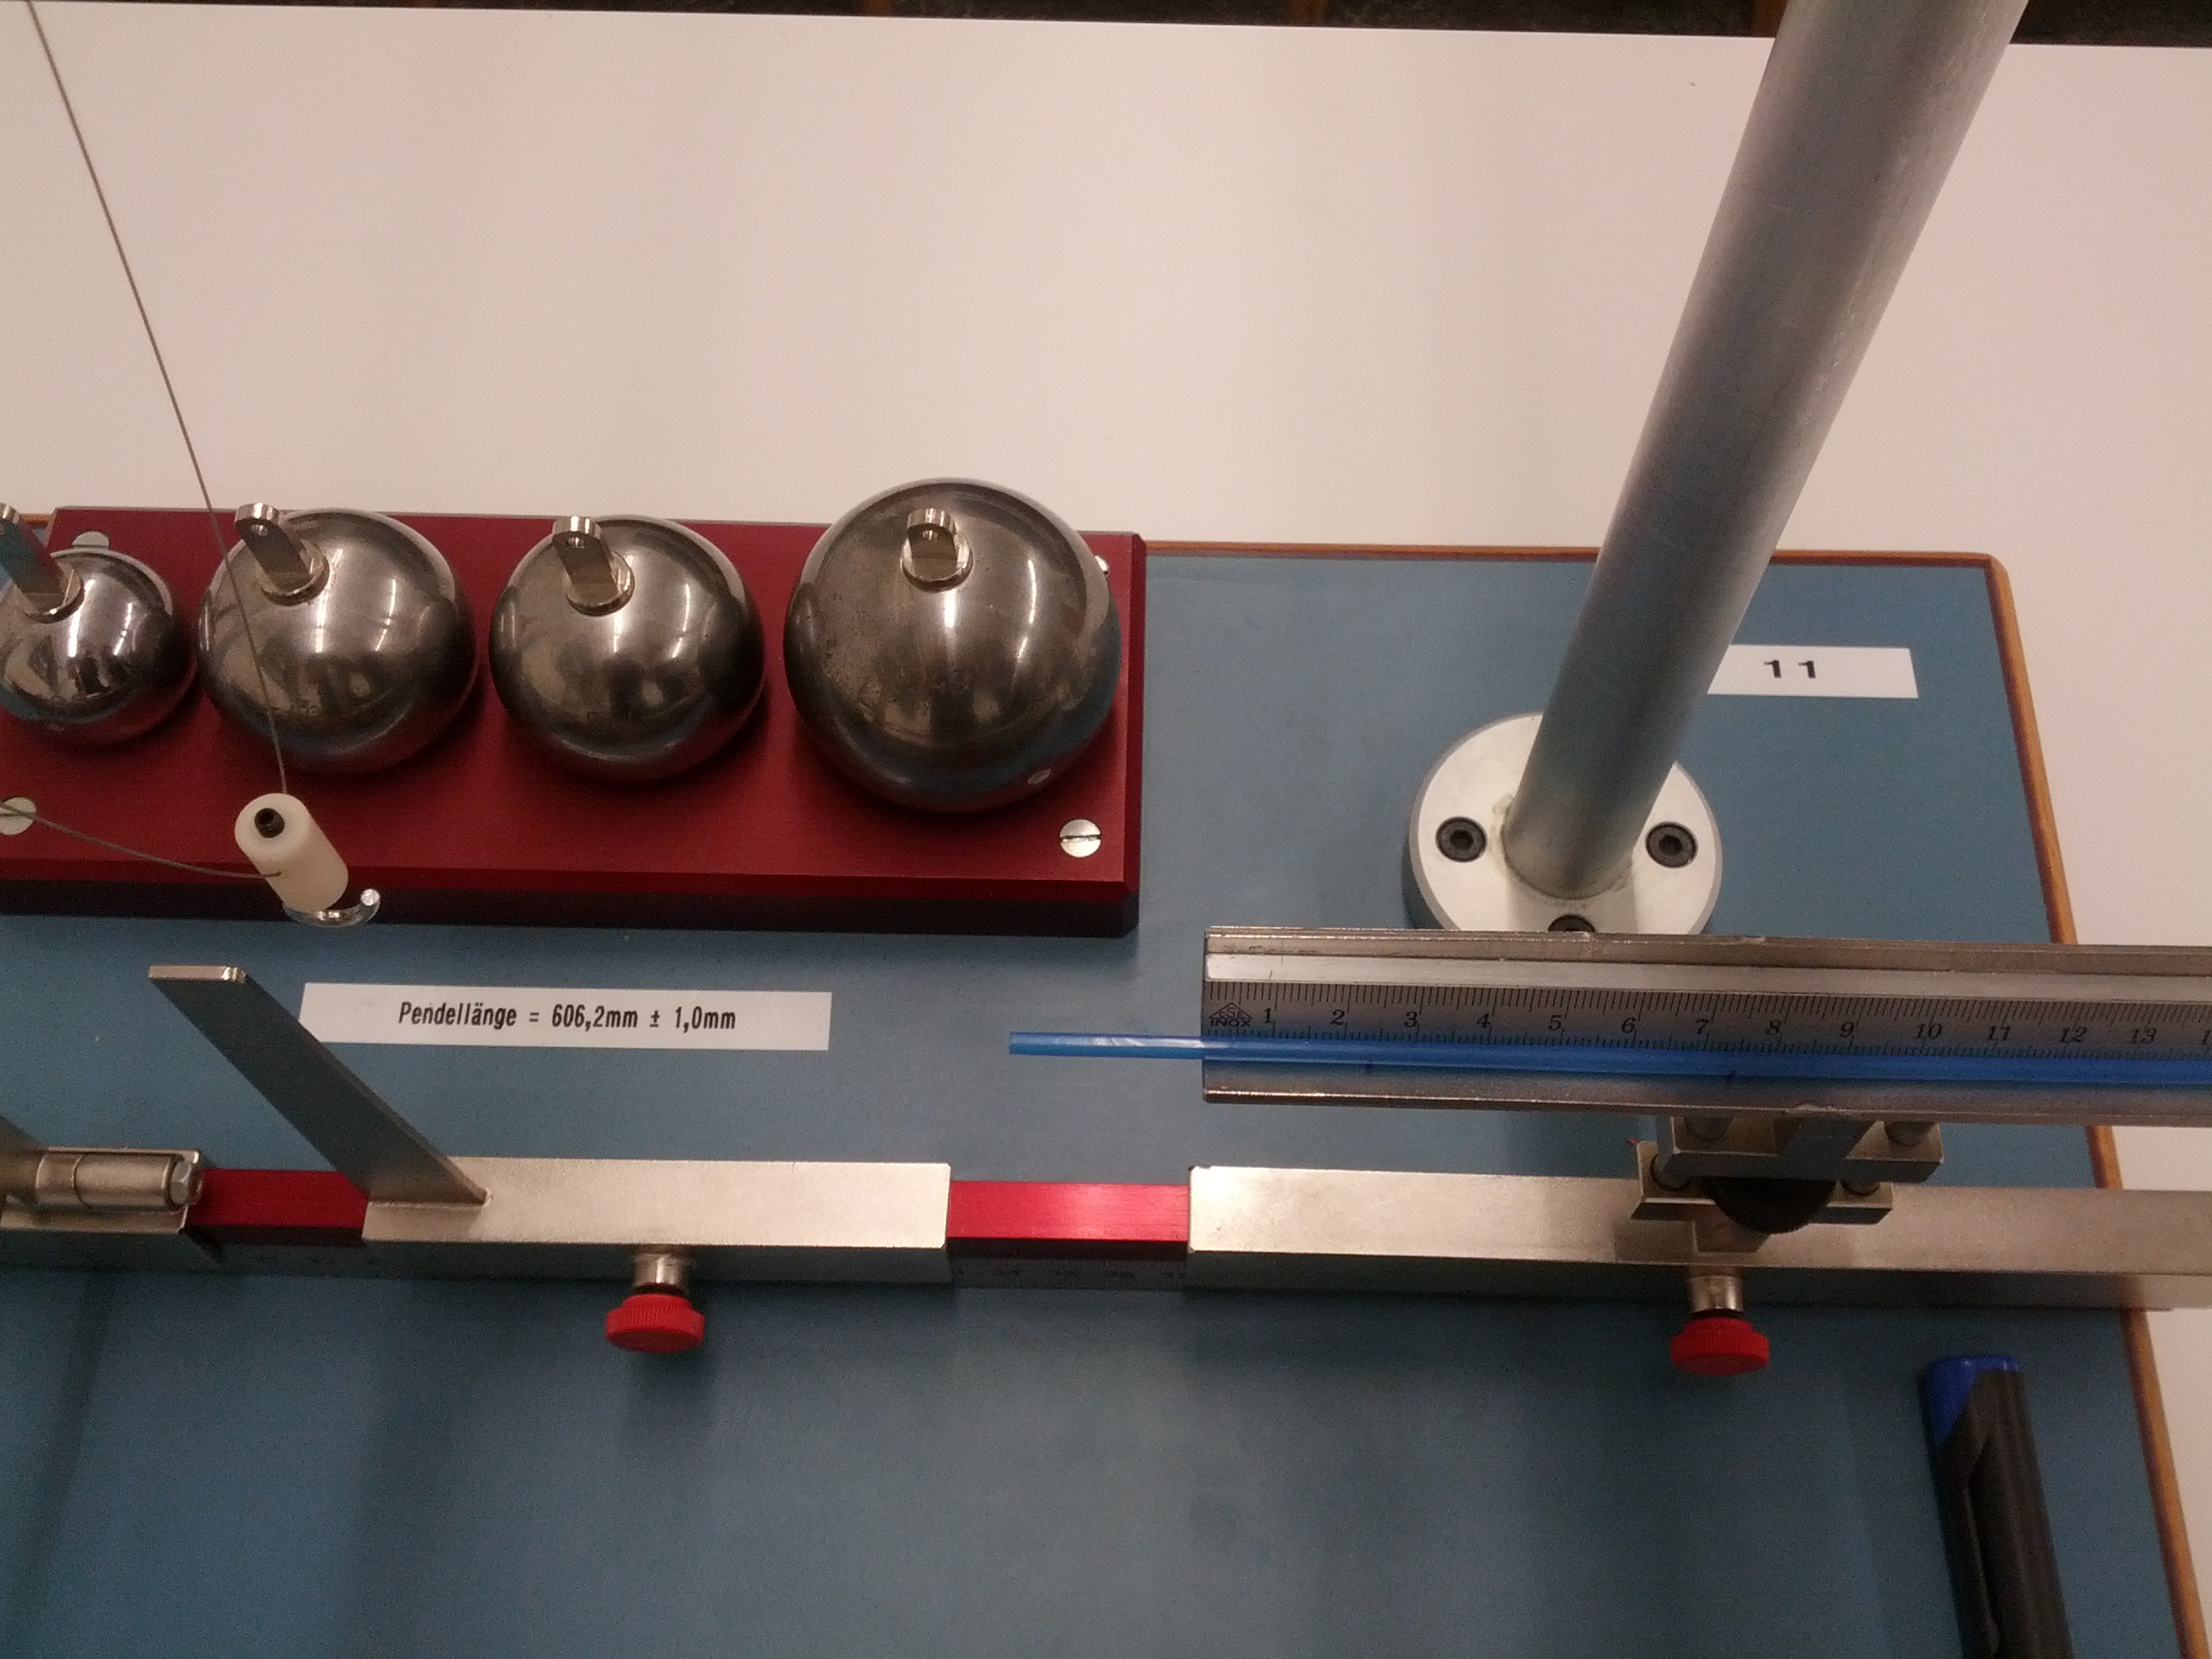
\includegraphics[width=0.9\textwidth]{img/topview.jpg}
	\caption{All used materials}
	\label{fig:materials}
\end{figure}

\subsection{Assembly}
\begin{figure}[H]
	\centering
  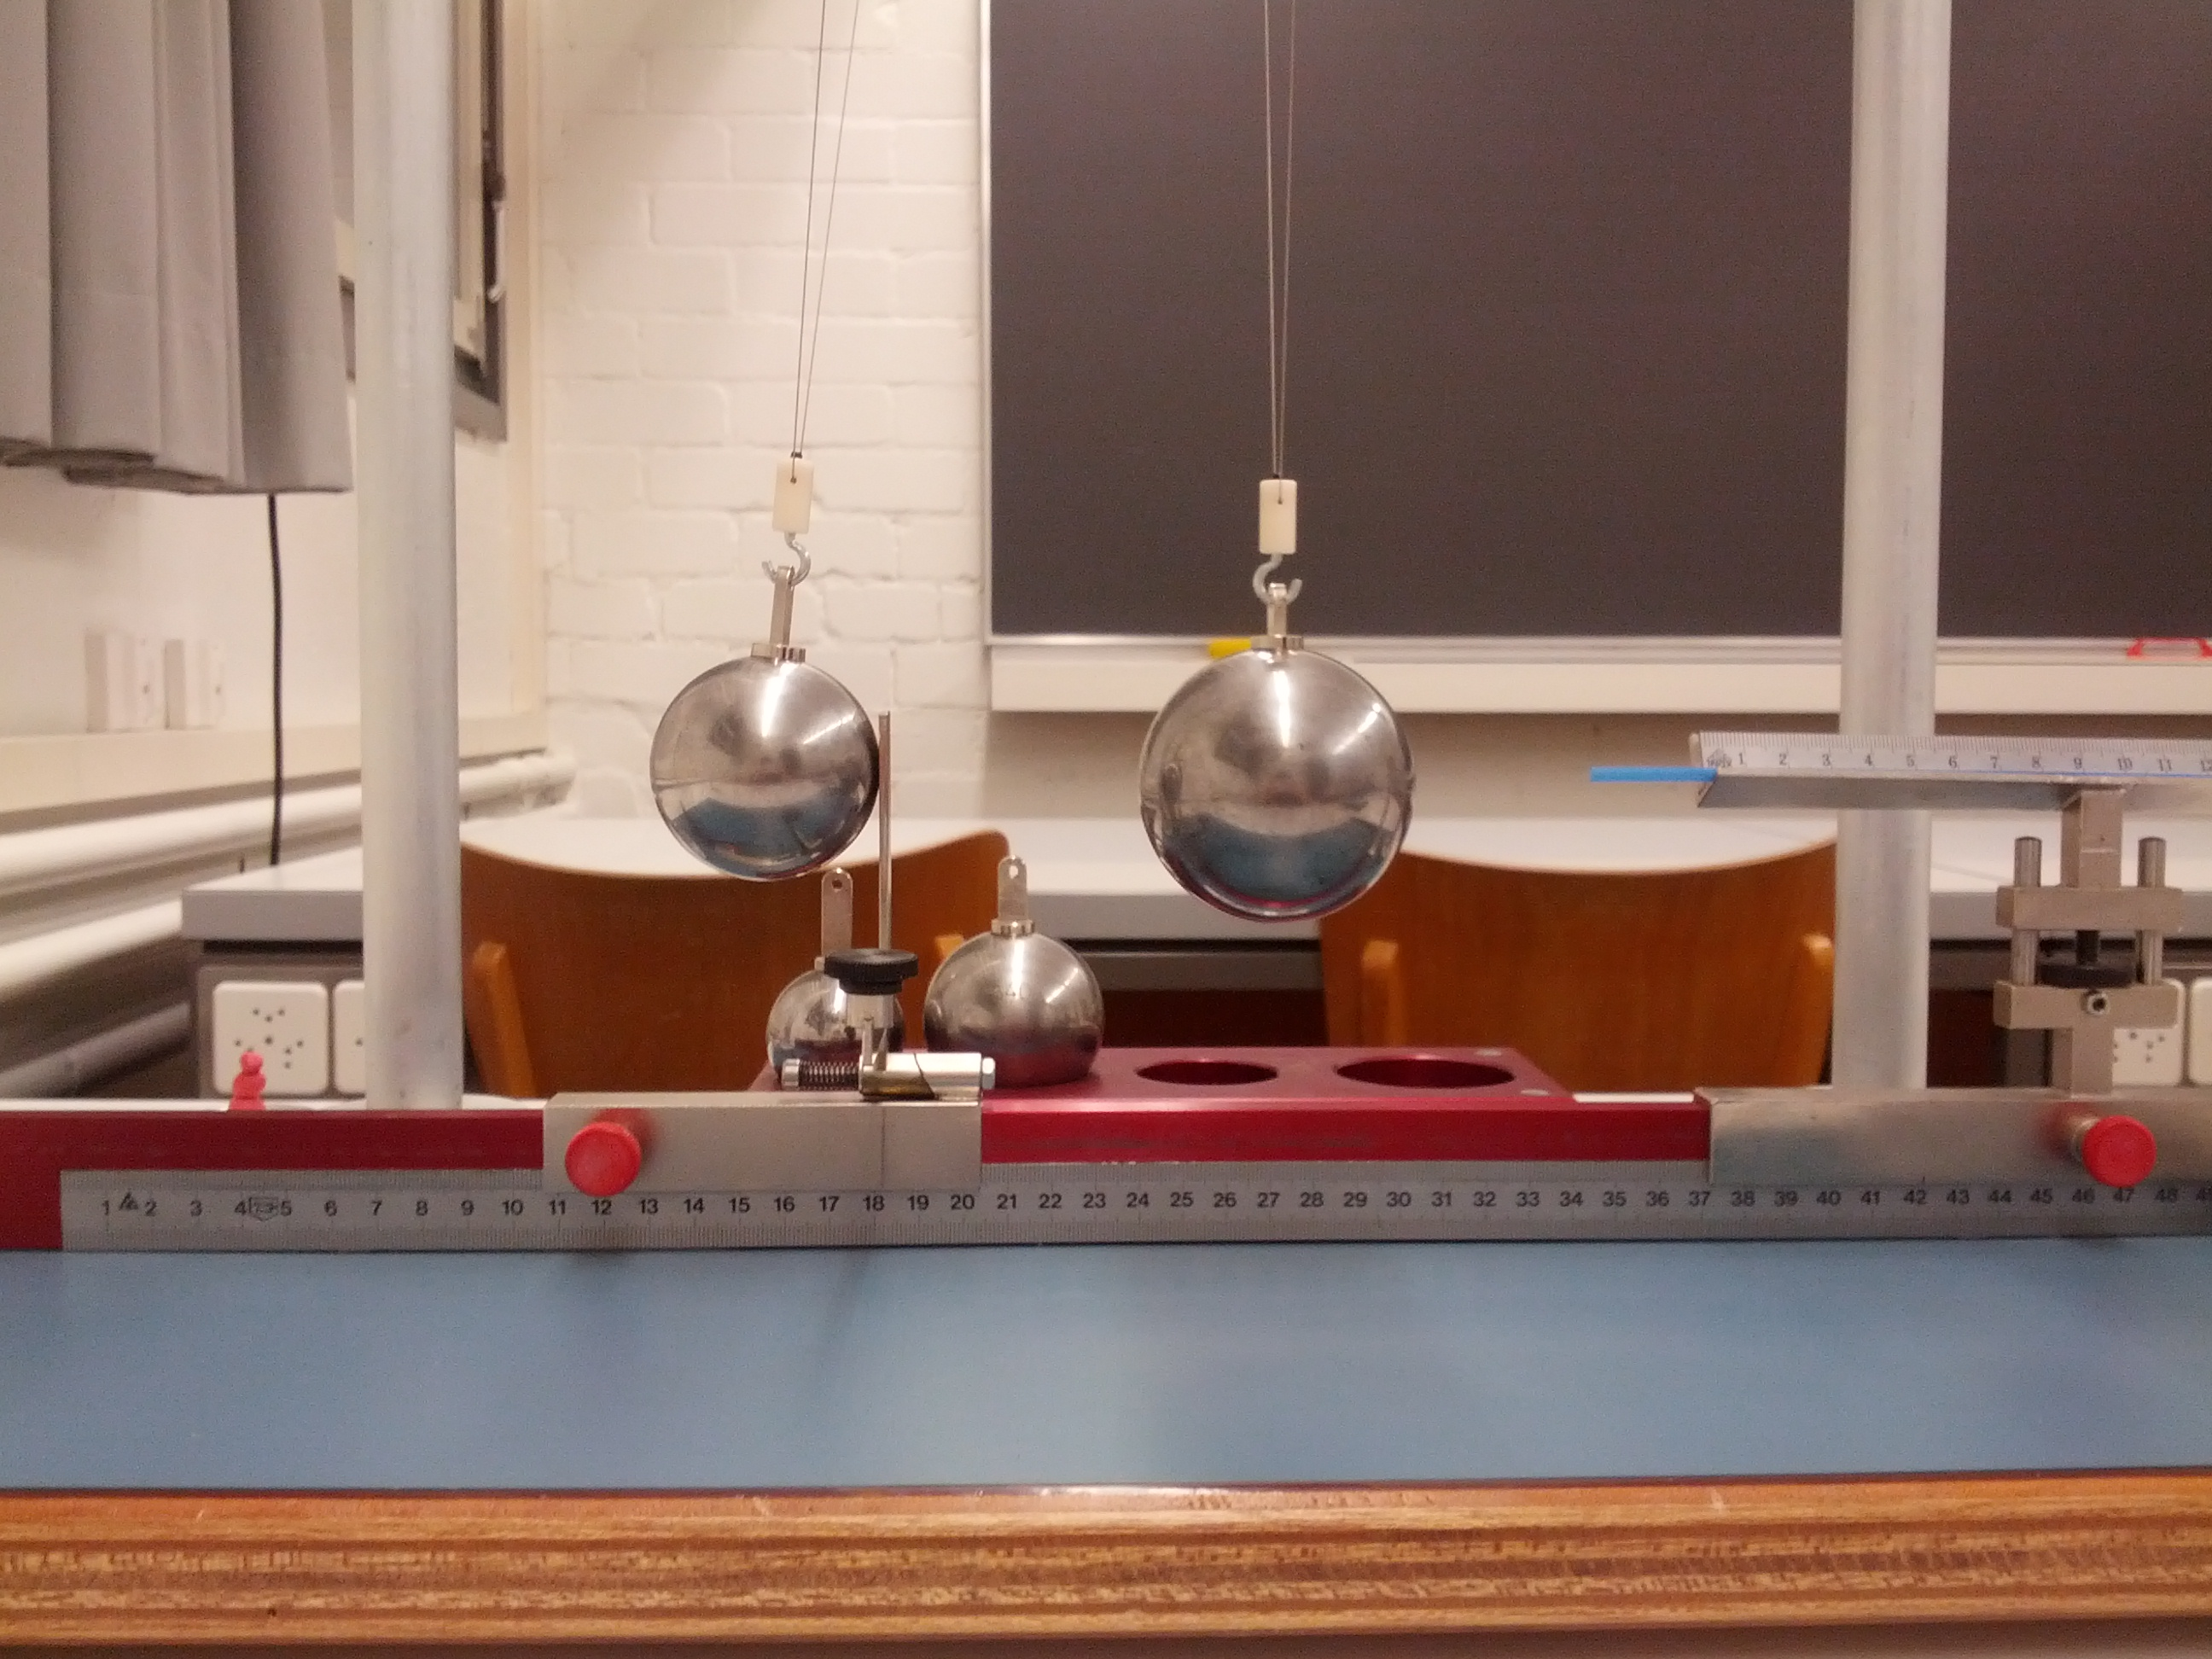
\includegraphics[width=0.9\textwidth]{img/assembly.jpg}
	\caption{Final experiment assembly}
	\label{fig:assembly}
\end{figure}

\section{Measurements}
\subsection{Elastic Collision}
\begin{table}[H]
	\centering
	\begin{tabular}{ccp{1.5cm}ccp{1.5cm}cc}
 P: 1 &   T: 2 &            &  P: 1 &   T: 3 &            &  P: 2 &   T: 1 \\\cline{1-2}\cline{4-5}\cline{7-8}

     159 &         93 &            &      158 &         56 &            &         86 &         114 \\
     159 &         93 &            &      158 &         56 &            &         86 &         115 \\
     159 &         94 &            &      158 &         55 &            &         86 &         115 \\
     159 &         94 &            &      158 &         55.5 &          &         86 &         114.5 \\
     159 &         95 &            &      158 &         55.5 &          &         86 &         114 \\
     159 &         93 &            &      158 &         55.5 &          &         86 &         114 \\
     159 &         93 &            &      158 &         55 &            &         86 &         114.5 \\
     159 &         93 &            &      158 &         54.5 &          &         86 &         114.5 \\
     159 &         93 &            &      158 &         56 &            &         86 &         115 \\
     159 &         93 &            &      158 &         56 &            &         86 &         115 \\
         &            &            &            &            &            &            &            \\

 P: 2 &   T: 2 &            &  P: 2 &   T: 3 &            &  P: 3 &   T: 2 \\\cline{1-2}\cline{4-5}\cline{7-8}

     95 &         92 &            &      146 &         96.5 &            &         72.5 &         89.5 \\
     95 &         93 &            &      146 &         97.5 &            &         72.5 &         89.5 \\
     95 &         93 &            &      146 &         97.5 &            &         72.5 &         89.5 \\
     95 &         93 &            &      146 &         97 &              &         72.5 &         89.5 \\
     95 &         93 &            &      146 &         96.5 &            &         72.5 &         89.5 \\
     95 &         92.5 &          &      146 &         96.5 &            &         72.5 &         89.5 \\
     95 &         92 &            &      146 &         96.5 &            &         72.5 &         90 \\
     95 &         92 &            &      146 &         95 &              &         72.5 &         89.5 \\
     95 &         92.5 &          &      146 &         95.5 &            &         72.5 &         90 \\
     95 &         92 &            &      146 &         96.5 &            &         72.5 &         89.5 \\
           &         &            &            &            &            &            &            \\

 P: 3 &   T: 1 &            &            &            &            &            &            \\\cline{1-2}

     72.5 &         107.5 &            &            &            &            &            &            \\
     72.5 &         108.5 &            &            &            &            &            &            \\
     72.5 &         108 &            &            &            &            &            &            \\
     72.5 &         109.5 &            &            &            &            &            &            \\
     72.5 &         109.5 &            &            &            &            &            &            \\
     72.5 &         109.5 &            &            &            &            &            &            \\
     72.5 &         110.5 &            &            &            &            &            &            \\
     72.5 &         107.5 &            &            &            &            &            &            \\
     72.5 &         109.5 &            &            &            &            &            &            \\
     72.5 &         108.5 &            &            &            &            &            &            \\
\end{tabular}  
\caption{Measured defecletions in [$\unit{mm}$]} for all \emph{elastic} collisions. Initially deflected projectile 'P' hits resting target 'T'.   
\end{table}

\subsection{Inelastic Collision}
\begin{table}[H]
	\centering
	\begin{tabular}{ccp{1.5cm}ccp{1.5cm}cc}
 P: 1 &   T: 2 &            &  P: 1 &   T: 3 &            &  P: 2 &   T: 1 \\\cline{1-2}\cline{4-5}\cline{7-8}

     159 &         45 &            &      158 &         28 &            &         86 &         56 \\
     159 &         47 &            &      158 &         27 &            &         86 &         56.5 \\
     159 &         49 &            &      158 &         26 &            &         86 &         56.5 \\
     159 &         45 &            &      158 &         26 &          &         86 &         56 \\
     159 &         46 &            &      158 &         26.5 &          &         86 &         56 \\
     159 &         45 &            &      158 &         26 &          &         86 &         59 \\
     159 &         44 &            &      158 &         27 &            &         86 &         59 \\
     159 &         44 &            &      158 &         26.5 &          &         86 &         57.5 \\
     159 &         45 &            &      158 &         27 &            &         86 &         59 \\
     159 &         45 &            &      158 &         26 &            &         86 &         58 \\
         &            &            &            &            &            &            &            \\

 P: 2 &   T: 2 &            &  P: 2 &   T: 3 &            &  P: 3 &   T: 2 \\\cline{1-2}\cline{4-5}\cline{7-8}

     95 &         45 &            &      146 &         45.5 &            &         72.5 &         44.5 \\
     95 &         46 &            &      146 &         45.5 &            &         72.5 &         45 \\
     95 &         46 &            &      146 &         46.5 &            &         72.5 &         43.5 \\
     95 &         45 &            &      146 &         48 &              &         72.5 &         43.5 \\
     95 &         44 &            &      146 &         45.5 &            &         72.5 &         43.5 \\
     95 &         47.5 &          &      146 &         44.5 &            &         72.5 &         43.5 \\
     95 &         44 &            &      146 &         48 &            &         72.5 &         42.5 \\
     95 &         44 &            &      146 &         47 &              &         72.5 &        43.5 \\
     95 &         44.5 &          &      146 &         46.5 &            &         72.5 &         42.5 \\
     95 &         46.5 &            &      146 &         47 &            &         72.5 &         44 \\
           &         &            &            &            &            &            &            \\

 P: 3 &   T: 1 &            &            &            &            &            &            \\\cline{1-2}

     72.5 &         56.5 &            &            &            &            &            &            \\
     72.5 &         57.5 &            &            &            &            &            &            \\
     72.5 &         57 &            &            &            &            &            &            \\
     72.5 &         57.5 &            &            &            &            &            &            \\
     72.5 &         57 &            &            &            &            &            &            \\
     72.5 &         57 &            &            &            &            &            &            \\
     72.5 &         57 &            &            &            &            &            &            \\
     72.5 &         57 &            &            &            &            &            &            \\
     72.5 &         56.5 &            &            &            &            &            &            \\
     72.5 &         57 &            &            &            &            &            &            \\
\end{tabular}  
\caption{Measured defecletions in [$\unit{mm}$]} for all \emph{inelastic} collisions. Initially deflected projectile 'P' hits resting target 'T'.   
\end{table}

\section{Analysis and Discussion}
\subsection{Elastic Collision}
\begin{table}[H]
\centering
\begin{tabular}{r||rrrrrrr}
 \emph{elastic} &    1 on 2 &    1 on 3 &    2 on 1 &    2 on 2 &    2 on 3 &    3 on 2 &    3 on 1 \\\hline\hline
$m_1$ [kg] &      0.233 &      0.233 &      0.540 &      0.540 &      0.540 &      1.049 &      1.049 \\
$m_2$ [kg] &      0.540 &      1.049 &      0.233 &      0.540 &      1.049 &      0.540 &      0.233 \\
$A=\frac{m_2}{m_1}$ &      2.318 &      4.502 &      0.431 &      1.000 &      1.943 &      0.515 &      0.222 \\\hline
$\overline{a_1}$ [mm] &     159.000 &     158.000 &     86.000 &     95.000 &     146.000 &     72.500 &     72.500 \\
$\overline{a_2}$ [mm] &     93.400 &     55.500 &     114.550 &     92.500 &     96.500 &     89.600 &     108.850 \\
$s_{\overline{a_2}}$ &      0.221 &      0.167 &      0.138 &      0.149 &      0.247 &      0.067 &      0.317 \\\hline
$T_2'/T_1$ Theory &      0.842 &      0.595 &      0.842 &      1.000 &      0.897 &      0.897 &      0.595 \\
$\overline{t}=T_2'/T_1$ Meas. &      0.800 &      0.556 &      0.766 &      0.948 &      0.849 &      0.786 &      0.501 \\
$s_{\overline{t}}$ &     0.0205 &     0.0145 &      0.0357 &      0.0400 &      0.0237 &      0.0434 &      0.0278 \\
\end{tabular}  
\caption{Analysis for elastic collision}
\label{tab:resultat1}
\end{table}

\subsection{Inelastic Collision}

\begin{table}[H]
\centering
\begin{tabular}{r||rrrrrrr}
 \emph{inelastic} &    1 on 2 &    1 on 3 &    2 on 1 &    2 on 2 &    2 on 3 &    3 on 2 &    3 on 1 \\\hline\hline
$m_1$ [kg] &      0.233 &      0.233 &      0.540 &      0.540 &      0.540 &      1.049 &      1.049 \\
$m_2$ [kg] &      0.540 &      1.049 &      0.233 &      0.540 &      1.049 &      0.540 &      0.233 \\
$A=\frac{m_2}{m_1}$ &      2.318 &      4.502 &      0.431 &      1.000 &      1.943 &      0.515 &      0.222 \\\hline
$\overline{a_1}$ [mm] &     159.000 &     158.000 &     86.000 &     95.000 &     146.000 &     72.500 &     72.500 \\
$\overline{a_2}$ [mm] &     93.400 &     55.500 &     114.550 &     92.500 &     96.500 &     89.600 &     108.850 \\
$s_{\overline{a_2}}$ &      0.221 &      0.167 &      0.138 &      0.149 &      0.247 &      0.067 &      0.317 \\\hline
$T_2'/T_1$ Theory &      0.842 &      0.595 &      0.842 &      1.000 &      0.897 &      0.897 &      0.595 \\
$\overline{t}=T_2'/T_1$ Meas. &      0.800 &      0.556 &      0.766 &      0.948 &      0.849 &      0.786 &      0.501 \\
$s_{\overline{t}}$ &     0.0205 &     0.0145 &      0.0357 &      0.0400 &      0.0237 &      0.0434 &      0.0278 \\
\end{tabular}  
\caption{Results for inelastic collision}
\label{tab:resultat2}
\end{table}

\begin{figure}[H]
	\centering
  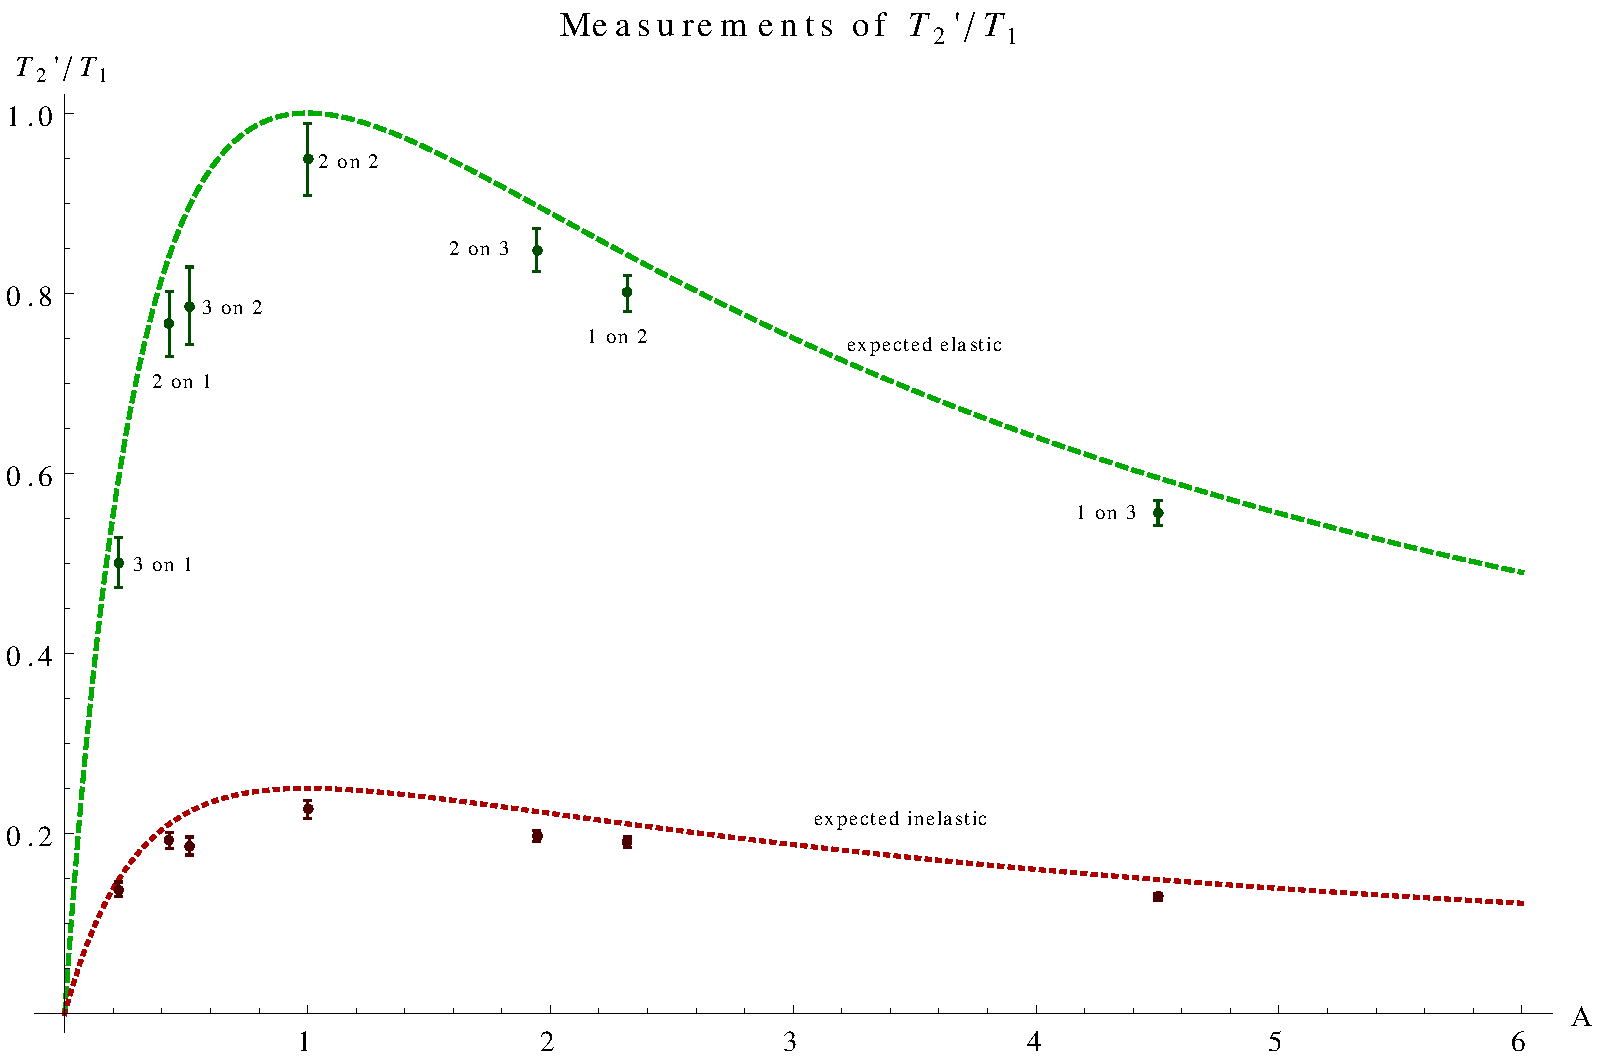
\includegraphics[width=1.0\textwidth]{diag/analysis.pdf}
	\caption{Consolidated analysis of both elastic and inelastic measurements}
	\label{fig:analysis}
\end{figure}
\begin{thebibliography}{9}

\bibitem{physcript13}
  Peter Wurz,
  \emph{Anleitung zum Physikpraktikum}
  FS2013

\end{thebibliography}

\end{document}
